\section{The solar resource and its ceiling}
\label{sec:resource}

\paragraph{From the solar constant to the surface.} A disk of Earth's radius
intercepts $S_0 \pi R^2 \approx \InterceptedTW~\mathrm{TW}$. Spreading that over
the rotating sphere and averaging over day and night divides the peak
irradiance $S_0$ by four, giving a top-of-atmosphere (TOA) horizontal mean of
$\ToaMean~\mathrm{W/m^2}$ --- a value our model reproduces from the daily
insolation integral to within $0.5~\mathrm{W/m^2}$. The atmosphere then takes
its share: clouds and aerosols reflect about a quarter back to space, the ozone
layer absorbs roughly \OzoneFrac\% (almost entirely in the ultraviolet), and
water vapour and aerosols absorb a further fifth, leaving a global-mean surface
irradiance of $\SurfaceGHI~\mathrm{W/m^2}$. Figure~\ref{fig:cascade} (left)
shows the full waterfall.

\paragraph{The ozone term.} The user's question singled out the ozone layer,
and it earns its place in the cascade for a reason disproportionate to its
\OzoneFrac\% energy share: it removes the biologically destructive UV-B/UV-C
band almost entirely. Energetically it is a minor loss; biologically it is the
precondition for there being surface ecosystems to share light with at all.

\paragraph{Where the resource is.} Insolation is not uniform. The equator
receives the most TOA radiation but sits under a persistent cloud belt; the
subtropical desert belt ($15$--$35^\circ$) combines high sun angles with the
clearest skies and is the true resource maximum, at
$\BestBandGHI~\mathrm{W/m^2}$ annual-mean surface irradiance
(Figure~\ref{fig:cascade}, right). This is why the feasibility analysis that
follows places panels in deserts, not on the equator.

\begin{figure}[t]
\centering
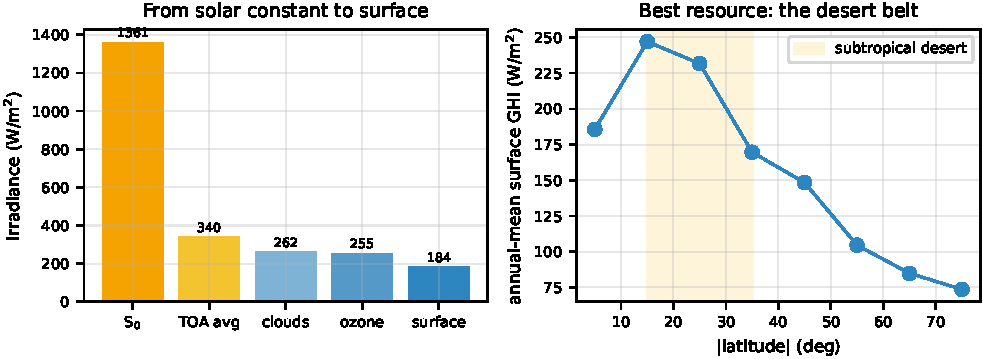
\includegraphics[width=\linewidth]{figures/cascade_bands.pdf}
\caption{\textbf{Left:} the loss cascade from the solar constant
($S_0$) through the TOA average, cloud reflection, ozone absorption, and
water/aerosol absorption to the surface global horizontal irradiance (GHI).
\textbf{Right:} annual-mean surface GHI by latitude band --- the subtropical
desert belt (shaded) is the resource maximum, not the equator.}
\label{fig:cascade}
\end{figure}
